\section{Configuration overview}
The mARGOt autotuning framework implements a Monitor-Analyze-Plan-Execute loop based on application knowledge (MAPE-K).
The application Knowledge describes the application behavior, by varying the selected software-knobs configuration and according to the input features.
In the mARGOt context, this knowledge is defined as a list of points, named Operating Points.
Each Operating Point relate the perfomance reached by the application using a given software-knobs configuration, in the context of the given input features.
The application knowledge might be derived at design-time, using a well-known algorithm to perform a Design Space Exploration, or at runtime, using a dedicated component (\prettyref{ssec:agora}).
The extra-functional concerns define the Monitor-Analyze-Plan-Execute, by specifying all the information required to instantiate a MAPE loop tailored for the target application.


From the integration point of view, we need to create at least one configuration file, written in json format, to enable the high-level interface generation.
In particular, all the extra-functional concerns of all the blocks that compose the application, must be written in a single file.
\prettyref{sec:adaptation} describes in detatils its semantic and systax.
Then, if we have gathered the application knowledge at design time, we need to write one or more configartion files that describes the Operating Point list for each block managed by mARGOt.
\prettyref{sec:knowledge} describes in details the semantic and syntax of those files.

\begin{figure}
\centering
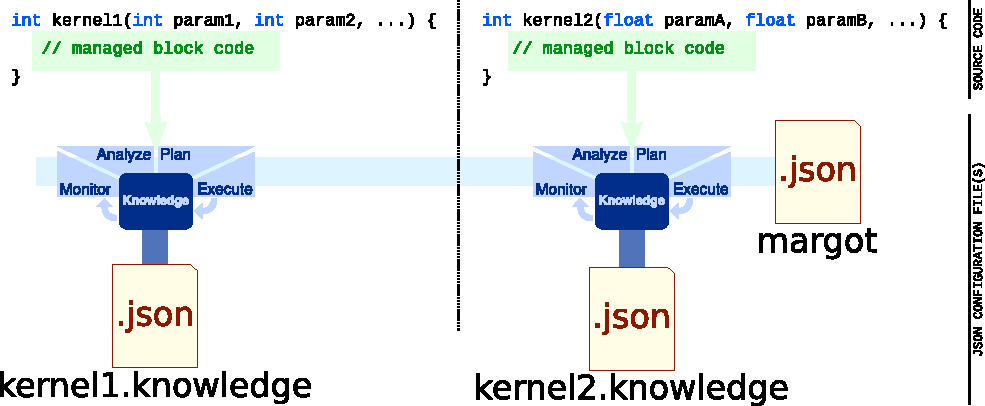
\includegraphics[scale=0.9]{manager}
\caption{Graphical representation of the relationship between configuration files and extra-functional concerns, in an application example.}
\label{fig:manager}
\end{figure}


To clarify the concept, \prettyref{fig:manager} shows an example of integration.
In particular, we suppose that the application is composed of two block of code managed by mARGOt, contained in two functions, named ``kernel1'' and ``kernel2''.
The two block of codes represent independent phases of the application, therefore they have completely different extra-functional requirements.
This leads to the instantiations of two different MAPE loops, based on knowledge, that drive the selection of two different set of software-knobs.
To generate this interface, it is required to write a configuration file (named ``margot.json'' in this example) with all the extra-functional concerns.
Then, we create a configuration file for each block, with the application knowledge (named ``kernelX.knowledge.json'' in this example).
